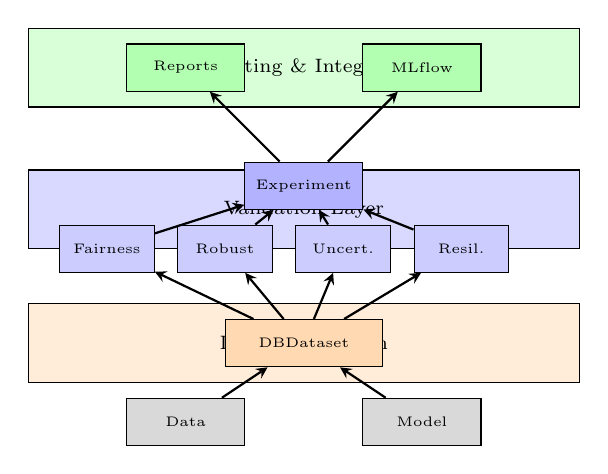
\begin{tikzpicture}[
    layer/.style={rectangle, draw, minimum width=7cm, minimum height=1cm, align=center, font=\scriptsize},
    component/.style={rectangle, draw, minimum width=1.5cm, minimum height=0.6cm, align=center, font=\tiny},
    arrow/.style={->, >=stealth, thick}
]

% Layer 3: Reporting
\node[layer, fill=green!15] (layer3) at (0,0) {Reporting \& Integration};
\node[component, fill=green!30] (report) at (-1.5,0) {Reports};
\node[component, fill=green!30] (mlflow) at (1.5,0) {MLflow};

% Layer 2: Validation
\node[layer, fill=blue!15] (layer2) at (0,-1.8) {Validation Layer};
\node[component, fill=blue!30] (exp) at (0,-1.5) {Experiment};
\node[component, fill=blue!20, minimum width=1.2cm] (f1) at (-2.5,-2.3) {Fairness};
\node[component, fill=blue!20, minimum width=1.2cm] (f2) at (-1,-2.3) {Robust};
\node[component, fill=blue!20, minimum width=1.2cm] (f3) at (0.5,-2.3) {Uncert.};
\node[component, fill=blue!20, minimum width=1.2cm] (f4) at (2,-2.3) {Resil.};

% Layer 1: Data
\node[layer, fill=orange!15] (layer1) at (0,-3.5) {Data Abstraction};
\node[component, fill=orange!30, minimum width=2cm] (db) at (0,-3.5) {DBDataset};

% Input
\node[component, fill=gray!30] (data) at (-1.5,-4.5) {Data};
\node[component, fill=gray!30] (model) at (1.5,-4.5) {Model};

% Arrows
\draw[arrow] (data) -- (db);
\draw[arrow] (model) -- (db);
\draw[arrow] (db) -- (f1);
\draw[arrow] (db) -- (f2);
\draw[arrow] (db) -- (f3);
\draw[arrow] (db) -- (f4);
\draw[arrow] (f1) -- (exp);
\draw[arrow] (f2) -- (exp);
\draw[arrow] (f3) -- (exp);
\draw[arrow] (f4) -- (exp);
\draw[arrow] (exp) -- (report);
\draw[arrow] (exp) -- (mlflow);

\end{tikzpicture}
